\documentclass[10.5pt,a4paper]{article}
\usepackage[utf8]{vietnam}
\usepackage{amsmath,amssymb}
\usepackage{tabularx}
\usepackage{tikz}
\usetikzlibrary{calc}
\usepackage[top=0.9cm, bottom=0.9cm, left=1.1cm, right=1.1cm]{geometry}
\usepackage{fancyhdr}
\usepackage{enumitem}

\pagestyle{fancy}
\fancyhf{}
\rfoot{\small\textit{Trang \thepage/2}}
\lfoot{\small\textit{Đề kiểm tra Giữa học kì I -- Môn Toán 7 -- Đề 1}}
\renewcommand{\headrulewidth}{0pt}

\setlength{\parskip}{0.5pt}

\begin{document}

\noindent
\begin{tabularx}{\linewidth}{X r}
\textbf{TRƯỜNG THCS \dots\dots\dots\dots\dots\dots} & \textbf{ĐỀ KIỂM TRA GIỮA HỌC KÌ I -- NĂM HỌC 2026 -- 2027} \\
\textbf{TỔ: \dots\dots\dots\dots\dots\dots} & \textbf{Môn: TOÁN -- Lớp 7} \\
\textit{(Đề 1 -- gồm 02 trang)} & \textit{Thời gian làm bài: 90 phút (không kể thời gian giao đề)} \\
\end{tabularx}

\vspace{1mm}
\noindent
\fbox{\parbox{\dimexpr\linewidth-2\fboxsep-2\fboxrule\relax}{
\textbf{Họ và tên học sinh:} \dots\dots\dots\dots\dots\dots\dots\dots\dots\dots\dots\dots\dots\dots\dots \textbf{Lớp:} \dots\dots\dots \textbf{Số báo danh:} \dots\dots\dots
}}

\vspace{1.5mm}
\noindent\textbf{\large PHẦN I. Câu trắc nghiệm nhiều phương án lựa chọn (3,0 điểm).}
\vspace{0.5mm}

\noindent\textit{Thí sinh trả lời từ câu 1 đến câu 12. Mỗi câu hỏi thí sinh chỉ chọn một phương án.}

\vspace{1mm}
\noindent\textbf{Câu 1.} Khẳng định nào sau đây đúng?\\
\begin{tabularx}{\linewidth}{X X X X}
A. $\dfrac{2}{3} \in \mathbb{Z}$ & B. $-\dfrac{3}{5} \in \mathbb{Q}$ & C. $-5 \notin \mathbb{Q}$ & D. $0,5 \notin \mathbb{Q}$
\end{tabularx}

\vspace{1mm}
\noindent\textbf{Câu 2.} Số đối của số hữu tỉ $-\dfrac{4}{7}$ là\\
\begin{tabularx}{\linewidth}{X X X X}
A. $\dfrac{4}{7}$ & B. $-\dfrac{4}{7}$ & C. $\dfrac{7}{4}$ & D. $-\dfrac{7}{4}$
\end{tabularx}

\vspace{1mm}
\noindent\textbf{Câu 3.} Với $x$ là số hữu tỉ khác 0, tích $x^5 \cdot x^3$ bằng\\
\begin{tabularx}{\linewidth}{X X X X}
A. $x^{15}$ & B. $x^2$ & C. $2x^8$ & D. $x^8$
\end{tabularx}

\vspace{1mm}
\noindent\textbf{Câu 4.} Áp dụng quy tắc chuyển vế, từ đẳng thức $x + \dfrac{1}{2} = \dfrac{3}{4}$ ta được\\
\begin{tabularx}{\linewidth}{X X X X}
A. $x = \dfrac{3}{4} + \dfrac{1}{2}$ & B. $x = \dfrac{1}{2} - \dfrac{3}{4}$ & C. $x = \dfrac{3}{4} - \dfrac{1}{2}$ & D. $x = \dfrac{3}{4} \cdot \dfrac{1}{2}$
\end{tabularx}

\vspace{1mm}
\noindent\textbf{Câu 5.} Phân số nào sau đây viết được dưới dạng số thập phân vô hạn tuần hoàn?\\
\begin{tabularx}{\linewidth}{X X X X}
A. $\dfrac{3}{8}$ & B. $\dfrac{5}{12}$ & C. $\dfrac{7}{20}$ & D. $\dfrac{9}{25}$
\end{tabularx}

\vspace{1mm}
\noindent\textbf{Câu 6.} Căn bậc hai số học của 64 là\\
\begin{tabularx}{\linewidth}{X X X X}
A. $8$ & B. $-8$ & C. $32$ & D. $8$ và $-8$
\end{tabularx}

\vspace{1mm}
\noindent\textbf{Câu 7.} Số nào sau đây là số vô tỉ?\\
\begin{tabularx}{\linewidth}{X X X X}
A. $\sqrt{9}$ & B. $-0,(3)$ & C. $\dfrac{2}{7}$ & D. $\sqrt{5}$
\end{tabularx}

\vspace{1mm}
\noindent\textbf{Câu 8.} Làm tròn số $3,14159$ với độ chính xác $0,005$ ta được\\
\begin{tabularx}{\linewidth}{X X X X}
A. $3,141$ & B. $3,15$ & C. $3,14$ & D. $3,1$
\end{tabularx}

\vspace{1mm}
\noindent\textbf{Câu 9.} Hai góc đối đỉnh thì\\
\begin{tabularx}{\linewidth}{X X X X}
A. bù nhau. & B. bằng nhau. & C. phụ nhau. & D. kề nhau.
\end{tabularx}

\vspace{1mm}
\noindent\textbf{Câu 10.} Qua một điểm $M$ nằm ngoài đường thẳng $a$, có bao nhiêu đường thẳng song song với $a$?\\
\begin{tabularx}{\linewidth}{X X X X}
A. Không có. & B. Có hai. & C. Có vô số. & D. Chỉ có một.
\end{tabularx}

\vspace{1mm}
\noindent
\begin{minipage}[m]{0.65\linewidth}
\textbf{Câu 11.} Cho hình bên, biết $\widehat{xOy} = 110^\circ$. Số đo góc $yOx'$ là\\
\begin{tabularx}{\linewidth}{X X}
A. $70^\circ$ & B. $110^\circ$ \\
C. $90^\circ$ & D. $20^\circ$
\end{tabularx}
\end{minipage}
\hfill
\begin{minipage}[m]{0.33\linewidth}
\centering
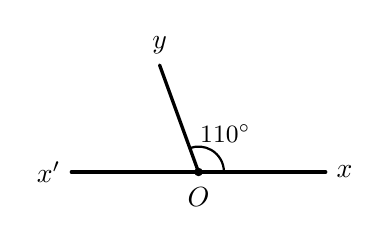
\begin{tikzpicture}[scale=0.85, line cap=round, line join=round]
  \coordinate (O) at (0,0);
  \coordinate (X) at (1.9,0);
  \coordinate (Xp) at (-1.9,0);
  \coordinate (Y) at ({1.7*cos(110)}, {1.7*sin(110)});
  \draw[very thick] (Xp) node[left] {$x'$} -- (X) node[right] {$x$};
  \draw[very thick] (O) -- (Y) node[above] {$y$};
  \fill (O) circle (1.8pt) node[below=2pt] {$O$};
  \draw[thick] (0.38,0) arc (0:110:0.38);
  \node at (55:0.7) {\small $110^\circ$};
\end{tikzpicture}
\end{minipage}

\vspace{1mm}
\noindent
\begin{minipage}[m]{0.65\linewidth}
\textbf{Câu 12.} Cho hình bên, đường thẳng $c$ cắt hai đường thẳng $a, b$ lần lượt tại $A, B$. Cặp góc nào sau đây là cặp góc so le trong?\\
\begin{tabularx}{\linewidth}{X X}
A. $\widehat{A}_1$ và $\widehat{B}_1$ & B. $\widehat{A}_4$ và $\widehat{B}_1$ \\
C. $\widehat{A}_4$ và $\widehat{B}_2$ & D. $\widehat{A}_2$ và $\widehat{A}_4$
\end{tabularx}
\end{minipage}
\hfill
\begin{minipage}[m]{0.33\linewidth}
\centering
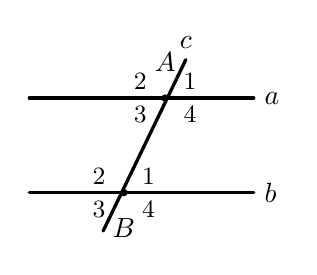
\begin{tikzpicture}[scale=0.75, line cap=round, line join=round]
  \draw[very thick] (-1.9, 0.9) -- (1.9, 0.9) node[right] {$a$};
  \draw[very thick] (-1.9, -0.7) -- (1.9, -0.7) node[right] {$b$};
  \coordinate (A) at (0.4, 0.9);
  \coordinate (B) at (-0.3, -0.7);
  \draw[very thick] ($ (B) - (0.35, 0.65) $) -- ($ (A) + (0.35, 0.65) $) node[above] {$c$};
  \fill (A) circle (1.8pt);
  \fill (B) circle (1.8pt);
  \node[above=6pt] at (A) {$A$};
  \node[below=6pt] at (B) {$B$};
  \node at ($ (A) + (0.42, 0.28) $) {\small $1$};
  \node at ($ (A) + (-0.42, 0.28) $) {\small $2$};
  \node at ($ (A) + (-0.42, -0.28) $) {\small $3$};
  \node at ($ (A) + (0.42, -0.28) $) {\small $4$};
  \node at ($ (B) + (0.42, 0.28) $) {\small $1$};
  \node at ($ (B) + (-0.42, 0.28) $) {\small $2$};
  \node at ($ (B) + (-0.42, -0.28) $) {\small $3$};
  \node at ($ (B) + (0.42, -0.28) $) {\small $4$};
\end{tikzpicture}
\end{minipage}

\newpage
\noindent\textbf{\large PHẦN II. Câu trắc nghiệm đúng sai (2,0 điểm).}
\vspace{0.5mm}

\noindent\textit{Thí sinh trả lời từ câu 13 đến câu 14. Trong mỗi ý a), b), c), d) ở mỗi câu, thí sinh chọn đúng hoặc sai.}

\vspace{1mm}
\noindent\textbf{Câu 13.} Cho các số thực $a = \sqrt{2}$; $b = -\dfrac{5}{3}$; $c = 1,(3)$; $d = |-1,5|$.\\
\begin{tabularx}{\linewidth}{X X}
\textbf{a)} $a$ là số hữu tỉ. & \textbf{b)} $c$ là số thập phân VHTH có chu kì là 3. \\
\textbf{c)} $b < d < a$. & \textbf{d)} Giá trị của $x$ thỏa mãn $\left|x - \dfrac{1}{2}\right| = d$ là $x = 2$ và $x = -1$.
\end{tabularx}

\vspace{1mm}
\noindent
\begin{minipage}[m]{0.65\linewidth}
\textbf{Câu 14.} Cho hình bên, đường thẳng $a$ và $b$ cùng vuông góc với $c$; đường thẳng $d$ cắt $a, b$ tại $M, N$ và $\widehat{M}_1 = 50^\circ$.\\
\textbf{a)} $\widehat{M}_3 = 50^\circ$.\hfill\textbf{b)} $a \parallel b$.\\
\textbf{c)} $\widehat{N}_2 = 50^\circ$.\hfill\textbf{d)} Tia phân giác góc $M_3$ cắt $b$ tại $P$. Khi đó $\widehat{MPN} = 50^\circ$.
\end{minipage}
\hfill
\begin{minipage}[m]{0.33\linewidth}
\centering
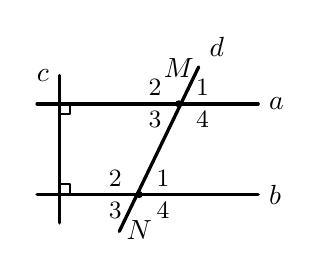
\begin{tikzpicture}[scale=0.72, line cap=round, line join=round]
  \draw[very thick] (-1.7, -1.2) -- (-1.7, 1.4) node[left] {$c$};
  \draw[very thick] (-2.1, 0.9) -- (1.8, 0.9) node[right] {$a$};
  \draw[very thick] (-2.1, -0.7) -- (1.8, -0.7) node[right] {$b$};
  \draw[thick] (-1.7, 0.9) rectangle ++(0.18, -0.18);
  \draw[thick] (-1.7, -0.7) rectangle ++(0.18, 0.18);
  \coordinate (M) at (0.4, 0.9);
  \coordinate (N) at (-0.3, -0.7);
  \draw[very thick] ($ (N) - (0.35, 0.65) $) -- ($ (M) + (0.35, 0.65) $) node[above right] {$d$};
  \fill (M) circle (1.8pt);
  \fill (N) circle (1.8pt);
  \node[above=6pt] at (M) {$M$};
  \node[below=6pt] at (N) {$N$};
  \node at ($ (M) + (0.42, 0.28) $) {\small $1$};
  \node at ($ (M) + (-0.42, 0.28) $) {\small $2$};
  \node at ($ (M) + (-0.42, -0.28) $) {\small $3$};
  \node at ($ (M) + (0.42, -0.28) $) {\small $4$};
  \node at ($ (N) + (0.42, 0.28) $) {\small $1$};
  \node at ($ (N) + (-0.42, 0.28) $) {\small $2$};
  \node at ($ (N) + (-0.42, -0.28) $) {\small $3$};
  \node at ($ (N) + (0.42, -0.28) $) {\small $4$};
\end{tikzpicture}
\end{minipage}

\vspace{1.5mm}
\noindent\textbf{\large PHẦN III. Câu trắc nghiệm trả lời ngắn (2,0 điểm).}
\vspace{0.5mm}

\noindent\textit{Thí sinh trả lời từ câu 15 đến câu 18.}

\vspace{1mm}
\noindent\textbf{Câu 15.} Tính giá trị của biểu thức $\sqrt{49} - \sqrt{16}$.\hfill
\textbf{Câu 16.} Tìm $x$, biết $\dfrac{3}{5}x + \dfrac{1}{4} = -\dfrac{7}{20}$.

\vspace{1mm}
\noindent
\begin{minipage}[m]{0.65\linewidth}
\textbf{Câu 17.} Cho hình bên, biết $a \parallel b$, đường thẳng $c$ cắt $a, b$ lần lượt tại $E, F$ và $\widehat{E}_1 = 72^\circ$. Tính số đo góc $F_2$ (đơn vị: độ).\\
\textbf{Câu 18.} Một mảnh vườn hình vuông có diện tích $150\text{ m}^2$. Bác An làm hàng rào bao quanh mảnh vườn (không để lối đi). Tính độ dài hàng rào (đơn vị: mét, làm tròn đến hàng đơn vị).
\end{minipage}
\hfill
\begin{minipage}[m]{0.33\linewidth}
\centering
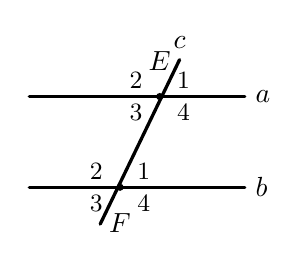
\begin{tikzpicture}[scale=0.72, line cap=round, line join=round]
  \draw[very thick] (-1.9, 0.9) -- (1.9, 0.9) node[right] {$a$};
  \draw[very thick] (-1.9, -0.7) -- (1.9, -0.7) node[right] {$b$};
  \coordinate (E) at (0.4, 0.9);
  \coordinate (F) at (-0.3, -0.7);
  \draw[very thick] ($ (F) - (0.35, 0.65) $) -- ($ (E) + (0.35, 0.65) $) node[above] {$c$};
  \fill (E) circle (1.8pt);
  \fill (F) circle (1.8pt);
  \node[above=6pt] at (E) {$E$};
  \node[below=6pt] at (F) {$F$};
  \node at ($ (E) + (0.42, 0.28) $) {\small $1$};
  \node at ($ (E) + (-0.42, 0.28) $) {\small $2$};
  \node at ($ (E) + (-0.42, -0.28) $) {\small $3$};
  \node at ($ (E) + (0.42, -0.28) $) {\small $4$};
  \node at ($ (F) + (0.42, 0.28) $) {\small $1$};
  \node at ($ (F) + (-0.42, 0.28) $) {\small $2$};
  \node at ($ (F) + (-0.42, -0.28) $) {\small $3$};
  \node at ($ (F) + (0.42, -0.28) $) {\small $4$};
\end{tikzpicture}
\end{minipage}

\vspace{1.5mm}
\noindent\textbf{\large PHẦN IV. Tự luận (3,0 điểm).}
\vspace{1mm}

\noindent\textbf{Câu 19 (1,0 điểm).} a) Tính hợp lí: $\dfrac{5}{7} \cdot \dfrac{3}{11} + \dfrac{5}{7} \cdot \dfrac{8}{11} - \dfrac{12}{7}$. \quad b) Tìm $x$, biết $\left(x - \dfrac{1}{2}\right)^2 = \dfrac{9}{16}$.

\vspace{1mm}
\noindent\textbf{Câu 20 (1,0 điểm).} Một cửa hàng nhập về $120\text{ kg}$ gạo. Ngày thứ nhất bán được $\dfrac{1}{4}$ số gạo, ngày thứ hai bán được $\dfrac{2}{3}$ số gạo còn lại.\\
\textbf{a)} Sau hai ngày, cửa hàng còn lại bao nhiêu ki-lô-gam gạo?\\
\textbf{b)} Ngày thứ ba, cửa hàng bán hết số gạo còn lại với giá giảm 10\% so với giá niêm yết là $18\,000$ đồng/kg. Tính số tiền cửa hàng thu được trong ngày thứ ba.

\vspace{1mm}
\noindent
\begin{minipage}[m]{0.64\linewidth}
\textbf{Câu 21 (1,0 điểm).} Cho hình bên, đường thẳng $AB$ cắt hai đường thẳng $xx'$ và $yy'$ lần lượt tại $A$ và $B$; biết $\widehat{xAB} = 120^\circ, \widehat{ABy} = 60^\circ$.\\
\textbf{a)} Chứng minh $xx' \parallel yy'$.\\
\textbf{b)} Vẽ tia $At$ là tia phân giác của góc $\widehat{xAB}$, tia $Bz$ là tia phân giác của góc $\widehat{ABy'}$ (như hình bên). Chứng minh $At \parallel Bz$.
\end{minipage}
\hfill
\begin{minipage}[m]{0.34\linewidth}
\centering
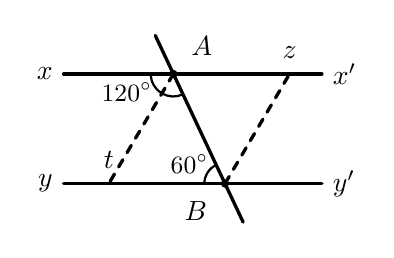
\begin{tikzpicture}[scale=0.82, line cap=round, line join=round]
  \coordinate (X) at (-2.0, 0.9);
  \coordinate (Xp) at (2.0, 0.9);
  \coordinate (Y) at (-2.0, -0.8);
  \coordinate (Yp) at (2.0, -0.8);
  \draw[very thick] (X) node[left] {$x$} -- (Xp) node[right] {$x'$};
  \draw[very thick] (Y) node[left] {$y$} -- (Yp) node[right] {$y'$};
  \coordinate (A) at (-0.3, 0.9);
  \coordinate (B) at (0.5, -0.8);
  \draw[very thick] ($ (A)!-0.35!(B) $) -- ($ (B)!-0.35!(A) $);
  \fill (A) circle (1.8pt) node[above right=3pt] {$A$};
  \fill (B) circle (1.8pt) node[below left=3pt] {$B$};
  \draw[thick] ($ (A) + (-0.35, 0) $) arc (180:295:0.35);
  \node at ($ (A) + (-0.72, -0.28) $) {\small $120^\circ$};
  \draw[thick] ($ (B) + (-0.32, 0) $) arc (180:115:0.32);
  \node at ($ (B) + (-0.55, 0.3) $) {\small $60^\circ$};
  \coordinate (T) at (-1.3, -0.8);
  \coordinate (Z) at (1.5, 0.9);
  \draw[very thick, dashed] (A) -- (T);
  \node[above=2pt] at (T) {$t$};
  \draw[very thick, dashed] (B) -- (Z);
  \node[above=2pt] at (Z) {$z$};
\end{tikzpicture}
\end{minipage}

\vfill
\begin{center}
\textbf{--------- HẾT ---------}\\
\textit{(Giáo viên coi kiểm tra không giải thích gì thêm)}
\end{center}

\end{document}
